\documentclass[a4paper,12pt]{article}
\usepackage[utf8]{inputenc}
\usepackage{graphicx}
\usepackage{amsmath}
\usepackage{hyperref}
\usepackage{enumitem}
\usepackage{biblatex}
\usepackage{pgf-umlsd}
\usepackage{parallel}
\usepackage{tikz}
\graphicspath{ {./img/} }
\usetikzlibrary{shapes.multipart}
\usetikzlibrary{positioning}
\usetikzlibrary{shadows}
\usetikzlibrary{calc}

\addbibresource{documentation.bib}


\title{An Evaluation of the current State of web server development in Rust and Java}
\author{Marc Matija}
\date{\today}
 
\begin{document}
	\maketitle
	\vspace{2cm}
	\begin{abstract}
		This paper aims to evaluate of the current state of web server development in Rust and Java. 
		In doing so, it will cover the basics of web server development in both languages, the tools and libraries 
		available, and the advantages and disadvantages of using each language for web server development. 
		Furthermore it will include a comparison of the two languages in terms of performance, ease of 
		use, and other factors that are important for web server development.
	\end{abstract}
	
	\newpage
	\tableofcontents
	\newpage
	
	\section{Introduction}
	\label{sec:introduction}
	Web server development is an important aspect of modern software development as they are 
	used to host websites, web applications, and other online services.
	One of the most popular languages for this is Java and the Spring framework.
	Java is a mature and widely used programming language that is known for its performance, scalability, and reliability.
	However, in recent years, Rust has emerged as a promising alternative to Java for web server development as seen at Discord 
	\cite{Discord}, Cloudflare\cite{Cloudflare_Pingora}, and other companies. 
	Rust is in stark contrast to Java, is a systems programming language that is designed for performance, safety, and concurrency.
	This paper aims to evaluate the current state of web server development in Rust and Java, and to provide an overview of 
	the tools, libraries, and best practices for web server development in both languages.
	
	\subsection{An Overview of Spring Boot}
	\label{subsec:spring_boot}
	Spring Boot is a popular Java framework for building web applications and microservices used by companies like 
	Deutsche Bahn\cite{DB_Job_Description}, Udemy \cite{Techstack_Udemy} and many others\cite{Spring_Boot_stackshare}.
	Built on top of the Spring framework, Spring Boot provides a set of tools and libraries that make it easy to build
	web applications and microservices in Java. It finds wide adoption in the industry due to its ease of use, maintanability 
	and scalability, aswell as the vast amount of libraries and tools available for it.

	\subsection{An Overview of Actix Web}
	\label{subsec:actix_web}
	Actix is a Rust framework for building backend services in rust and the one currently one of the most actively developed framworks,
	within the Rust ecosystem. It provides provides a very similar feature set to Spring Boot making it a suitable candidate for comparison.

	\newpage
	\subsection{Other Used Technologies}
	\label{subsec:used_technologies}
	In addition to the frameworks mentioned above, I will use the following technologies to build the web server:
	\begin{itemize}
		\item \textbf{PostgreSQL} \- A popular open-source relational database management system that is widely used in the industry.
		\item \textbf{Docker} \- A platform for building, shipping, and running applications in containers.
		\item \textbf{Docker Compose} \- A tool for defining and running multi-container Docker applications.
		\item \textbf{JWT} \- A standard for creating JSON-based access tokens that are used for authentication and authorization.
		\item \href{https://swagger.io/}{Swagger} \- A tool for designing, building, and documenting APIs.
		\item \href{https://junit.org/junit5/}{JUnit} \- A popular testing framework for Java.
		\item \textbf{Actix Web Test} \- A testing framework for Actix Web.
		\item \href{https://www.postman.com/}{Postman} \- A tool for testing APIs.
		\item \href{https://k6.io/}{K6} \- A tool for load testing web applications.
		\item \href{https://dbeaver.io/}{DBeaver} \- A database management tool.
	\end{itemize}

	\newpage
	\section{Specifications for the web server}
	\label{sec:example_project}
	In order to evaluate the current state of web server development in Rust and Java, I will build a simple web server in 
	both languages using the previously mentioned frameworks. The web server will feature a REST api that allows users to 
	create channels, add messages to channels, and retrieve messages from said channels. In addition, the web server will 
	feature a websocket endpoint that allows users to subscribe to channels and receive messages in real-time. Authentication 
	will be handled using JWT tokens and a profile endpoint to authenticate users and retrieve their information.

	\subsection{REST API}
	\label{subsec:rest_api}
	The REST API will feature the following endpoints:

	Channel endpoints:
	\begin{itemize}
		\item \textbf{Create Channel} \- POST /api/v1/channels \\
		Creates a new channel with the given name.
		\item \textbf{Get Channel} \- GET /api/v1/channels/\{id\} \\
		Retrieves the channel with the given id.
		\item \textbf{Get All Channels} \- GET /api/v1/channels \\
		Retrieves all channels.
		\item \textbf{Change Channel} \- PUT /api/v1/channels/\{id\} \\
		Changes the name of the channel with the given id.
		\item \textbf{Delete Channel} \- DELETE /api/v1/channels/\{id\} \\
		Deletes the channel with the given id.
	\end{itemize}

	Message endpoints:
	\begin{itemize}
		\item \textbf{Add Message} \- \texttt{ POST /api/v1/channels/\{id\}/messages } \\
		Adds a new message to the channel with the given id.
		\item \textbf{Get Message} \- \texttt{ GET /api/v1/channels/\{id\}/messages/\{id\} } \\
		Retrieves the message with the given id from the channel with the given id.
		\item \textbf{Get All Messages} \- \texttt{ GET /api/v1/channels/\{id\}/messages } \\
		Retrieves all messages from the channel with the given id.
		\item \textbf{Change Message} \- \texttt{ PUT /api/v1/channels/\{id\}/messages/\{id\} } \\
		Changes the content of the message with the given id from the channel with the given id.
		\item \textbf{Delete Message} \- \texttt{ DELETE /api/v1/channels/\{id\}/messages/\{id\}}
		Deletes the message with the given id from the channel with the given id.
	\end{itemize}

	Authentication endpoints:
	\begin{itemize}
		\item \textbf{Sign up} \texttt{ POST /api/v1/auth/signup } \\
		Registers a new user with the given username and password.
		\item \textbf{Sign in} \texttt{ POST /api/v1/auth/signin } \\
		Logs in the user with the given username and password.
		\item \textbf{Sign out} \texttt{ POST /api/v1/auth/signout } \\
		Logs out the currently logged in user.
	\end{itemize}

	Profile endpoints:
	\begin{itemize}
		\item \textbf{Get Profile} \texttt{ GET /api/v1/profile } \\
		Retrieves the profile of the currently logged in user.
		\item \textbf{Change Profile} \texttt{ PUT /api/v1/profile } \\
		Changes the profile of the currently logged in user.
		\item \textbf{Delete Profile} \texttt{ DELETE /api/v1/profile } \\
		Deletes the profile of the currently logged in user.
	\end{itemize}

	\newpage
	\subsection{Websocket API}
	\label{subsec:websocket_api}
	In order to allow users to recieve messages in real-time, the web server will feature a websocket endpoint that 
	allows users to subscribe to channels and receive updates when new messages are added to the channel. Users will
	automatically be subscribed to Channels they are a part of. When establishing a connection to a websocket endpoint,
	they will need to provide a valid JWT token in order to authenticate themselves.
	\begin{itemize}
		\item \textbf{Subscribe} \- \texttt{ws://localhost:8080/api/v1/ws} \\
		Subscribes the user to the websocket endpoint and allows them to receive updates when new messages are added
		to the channels they are a member of.
	\end{itemize}
	\begin{figure}[h]
		\caption[Message flow in a websocket connection]{Message flow in a websocket connection}
		\begin{sequencediagram}
			\renewcommand\unitfactor{0.6}
			\newthread{c}{Client}
			\newinst[1]{s}{Web Server}
			\begin{call}{c}{open()}{s}{}
				\begin{call}{c}{auth()}{s}{}
					\begin{call}{s}{verify()}{s}{}
					\end{call}
				\end{call}
				\begin{sdblock}{New Message}{}
					\begin{messcall}{s}{send()}{c}
					\end{messcall}
				\end{sdblock}
				\begin{messcall}{c}{close()}{s}{}
				\end{messcall}
			\end{call}
		\end{sequencediagram} \\
	\end{figure}
	
	In a websocket connection request, the headers of the HTTP request cannot be modified, the server will have to first 
	accept the connection, then wait for the client to send a JWT token. The server will then verify the token and if it is 
	valid, the client will be subscribed able to receive all messages from the channels they are a part of. Recieved 
	messages will take the same format as the messages in the REST API.


	\subsection{Database Schema}
	\label{subsec:database_schema}
	The Implementations in both languages will feature the same PostgreSQL database, thus the database schema will 
	be the same for both implementations.
	\begin{figure}[h]
		\centering
		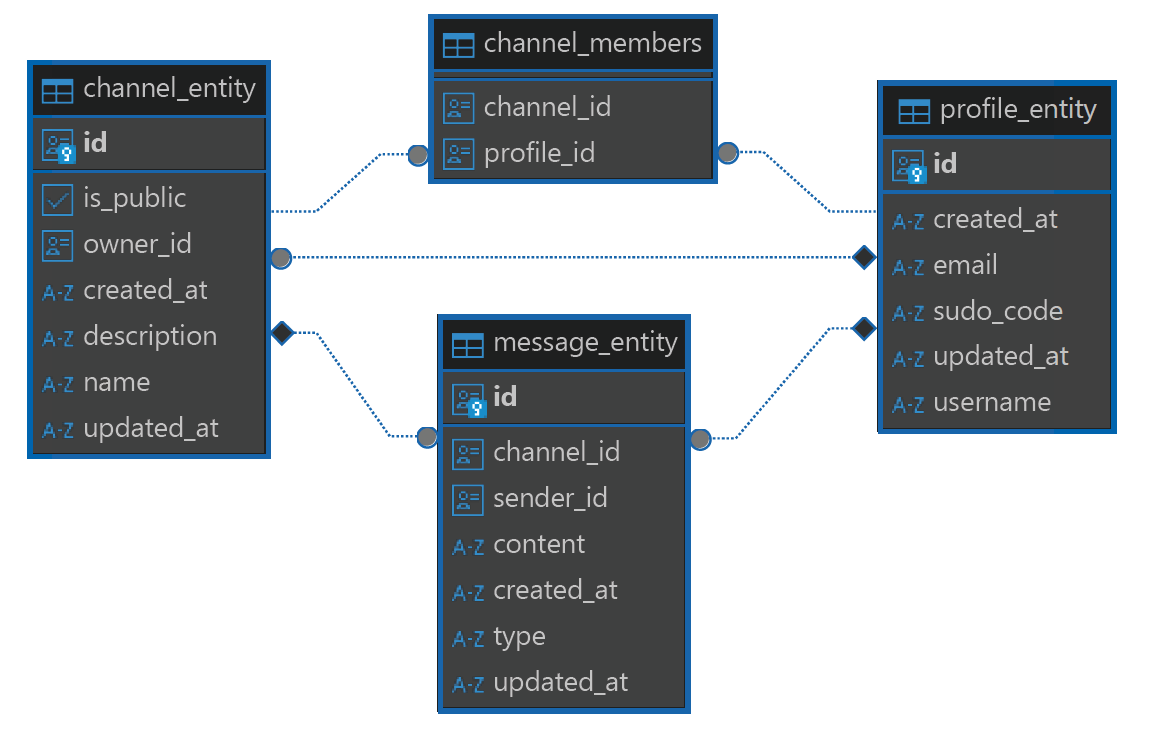
\includegraphics[width=\textwidth]{dbeaver_database_representation.png}
		\caption{Database schema in DBeaver}
		\label{fig:dbeaver_database_representation}
	\end{figure}
	
	It features a table for users, a table for channels, and a table for messages. The users table stores the username, email
	while the channels table stores the id of whoever created it, making him the \textbf{owner} of the channel. The messages table
	stores the content of the message, the id of the user who sent it, and the id of the channel it was sent to. All Tables also
	include coloumns for the creation and last update time of the row.

	\subsection{Authentication}
	\label{subsec:authentication}
	Authentication will be handled using JWT tokens. When a client signs up or signs in, they will receive a JWT token that
	they can use to authenticate themselves when making requests to the web server. The JWT token will be sent in the 
	Authorization header of the HTTP request as a Bearer token. Both Server implementations will have to verify the token 
	before sending new messages to the client.

	\section{Implementation in Java}
	\label{sec:java_implementation}

	\section{Implementation in Rust}
	\label{sec:rust_implementation}

	\section{Comparison}
	\label{sec:comparison}
	\subsection{Developer Experience}
	\subsection{Performance}
	
	\section{Conclusion}

	\newpage
	\section{Sources}
	\label{sec:Sources}
	\begin{itemize}
		\item \href{https://rust-edu.org/resources/}{Rust Edu}
		\item \href{https://doc.rust-lang.org/book/}{The Rust Programming Language}
		\item \href{https://doc.rust-lang.org/std/}{Rust Standard Library}
		\item \href{https://doc.rust-lang.org/cargo/}{Cargo Guide}
		\item \href{https://doc.rust-lang.org/rust-by-example/}{Rust by Example}
		\item \href{https://doc.rust-lang.org/rustdoc/}{Rustdoc}
		\item \href{https://actix.rs/}{Actix}
		\item \href{https://dbeaver.io/}{DBeaver}
	\end{itemize}
	\printbibliography[title={Whole bibliography}]
\end{document}